\chapter{La Pipeline di Rendering in Unity}

\section{Introduzione a HDRP}

La \textit{High Definition Render Pipeline} (HDRP) rappresenta l'approccio moderno di Unity per la gestione del rendering ad alta fedeltà, progettato specificamente per piattaforme hardware di fascia alta \cite{UnityHDRP}. A differenza della precedente \textit{Built-in Render Pipeline}, la HDRP non è un sistema statico, ma costituisce un'implementazione avanzata della \textit{Scriptable Render Pipeline} (SRP). 

L'architettura SRP introduce un cambio di paradigma fondamentale: il loop di rendering non è più codificato rigidamente all'interno del motore grafico, ma viene esposto tramite un'API C\#. Questo permette agli sviluppatori di estendere, modificare e ottimizzare il processo di disegno dei fotogrammi in base alle esigenze specifiche del progetto, un requisito essenziale per un lavoro di ottimizzazione mirato come quello richiesto da ARES \cite{GregoryGameEngine}.

Il pilastro filosofico della HDRP è il \textit{Physically Based Rendering} (PBR), un modello che mira a simulare l'interazione della luce con le superfici seguendo le leggi della fisica ottica \cite{PharrPBRT}. Per garantire tale coerenza, la pipeline opera esclusivamente in spazio colore lineare e utilizza calcoli in virgola mobile a 32 bit (FP32) \cite{AkenineRealTimeRendering}. Questo garantisce una gamma dinamica elevata (\textit{High Dynamic Range}), permettendo una gestione accurata di contrasti luminosi estremi e materiali complessi, ma introducendo al contempo un carico computazionale significativo che necessita di strategie di gestione della memoria e della GPU estremamente oculate.


\section{Gestione del carico computazionale}

Nel campo della computer grafica in tempo reale, la generazione di un fotogramma non dipende esclusivamente dalla potenza di calcolo della GPU, ma è il risultato di una complessa coordinazione tra quest'ultima e la CPU. Uno dei principali fattori che influenzano le prestazioni di un motore grafico come Unity è il numero di \textit{draw call} effettuate per ogni \textit{frame}.

\subsection{Il costo delle Draw Call}

Una \textit{draw call} può essere definita come un comando inviato dalla CPU alla GPU attraverso un'API grafica per istruire il processore grafico sul disegno di un determinato oggetto o di una porzione di geometria \cite{AkenineRealTimeRendering}. Sebbene la GPU sia estremamente efficiente nel processare migliaia di poligoni in parallelo, la preparazione di ogni singolo comando di disegno comporta un costo significativo per la CPU, noto come \textit{overhead} del driver \cite{GregoryGameEngine}.

Ogni volta che viene invocata una \textit{draw call}, il processore deve eseguire diverse operazioni preliminari:
\begin{itemize}
    \item Verificare lo stato della \textit{pipeline} di rendering.
    \item Impostare i parametri corretti all'interno della memoria della GPU.
    \item Tradurre i comandi del motore grafico in istruzioni comprensibili dal driver hardware.
\end{itemize}

Quando il numero di questi comandi è eccessivo, la CPU non riesce a prepararli con una velocità sufficiente a mantenere il \textit{frame rate} target, portando il sistema in una condizione di \textit{CPU-bound}. In questo scenario, la GPU rimane inattiva in attesa di istruzioni, causando cali di fluidità anche in presenza di hardware grafico di fascia alta.

\subsection{Cambiamenti di stato e SetPass Calls}

Oltre al numero assoluto di \textit{draw call}, un impatto determinante sulla fluidità è dato dai cambiamenti di stato della GPU (\textit{State Changes}). Ogni volta che un oggetto richiede un materiale, una \textit{texture} o uno \textit{shader} differente rispetto all'oggetto precedente, la GPU deve riconfigurare il proprio stato operativo \cite{AkenineRealTimeRendering, GregoryGameEngine}. 

Queste operazioni, spesso identificate in Unity come \textit{SetPass calls}, sono estremamente onerose. Una sequenza di \textit{draw call} che condividono lo stesso stato è molto più rapida da eseguire rispetto a una sequenza che richiede continui cambiamenti di configurazione. L'obiettivo dell'ottimizzazione grafica, dunque, non è solo la riduzione del numero di oggetti a schermo, ma la minimizzazione delle interazioni costose tra processore e scheda video attraverso tecniche di raggruppamento dei dati.

\section{Batching}

\subsection{Definizione}

Per ovviare ai limiti imposti dall'elevato numero di \textit{draw call}, la tecnica principale nel campo del \textit{real-time rendering} è il \textit{batching} \cite{AkenineRealTimeRendering}. Il termine definisce il processo di raggruppamento di più geometrie elementari in un unico blocco di dati da inviare alla GPU con un solo comando di disegno \cite{GregoryGameEngine}.

Il presupposto fondamentale affinché il \textit{batching} sia efficace è la condivisione dello stato di rendering. Due o più oggetti possono essere raggruppati in un unico \textit{batch} solo se condividono le medesime proprietà grafiche, tra cui:
\begin{itemize}
    \item Lo Shader: il programma che definisce come la luce interagisce con la superficie.
    \item Il Materiale: l'insieme dei parametri e delle \textit{texture} applicate all'oggetto.
    \item Le Texture: l'utilizzo di una singola risorsa immagine per più modelli 3D.
\end{itemize}

Attraverso il \textit{batching}, il carico computazionale viene spostato dalla preparazione di molti piccoli comandi alla gestione di pochi flussi di dati massivi. Questo approccio riduce drasticamente le interruzioni nel flusso di lavoro della GPU, poiché minimizza le \textit{SetPass calls} e permette al processore grafico di operare in modo continuo su grandi quantità di vertici.

\subsection{Batching in Unity}

Unity offre diverse strategie di \textit{batching} per far fronte all'ottimizzazione del rendering, ognuna con casi d'uso e limitazioni specifiche che devono essere valutate attentamente in fase di \textit{profiling}.

\subsection{Static Batching}

Dal punto di vista tecnico, lo \textit{static batching} agisce durante la fase di inizializzazione o di caricamento della scena. Il motore grafico analizza la geometria di tutti gli oggetti idonei e ne trasforma i vertici dalle rispettive coordinate locali (\textit{local space}) in un sistema di coordinate globale (\textit{world space}). Una volta ricalcolati, questi dati vengono concatenati in un unico, grande \textit{Vertex Buffer} e un relativo \textit{Index Buffer}. In questo modo, la CPU non deve più inviare istruzioni per ogni singolo oggetto, ma può istruire la GPU a renderizzare l'intero blocco di dati con un unico comando di disegno \cite{UnityStaticBatching}.

Sebbene questa tecnica garantisca un incremento notevole del \textit{frame rate} riducendo il carico sul processore, comporta un costo in termini di memoria RAM e VRAM superiore rispetto ad altre tecniche: poiché il motore deve memorizzare la nuova \textit{mesh} combinata oltre a quelle originali, l'occupazione di memoria cresce proporzionalmente alla complessità degli oggetti raggruppati.

Operativamente, all'interno dell'editor di Unity, il programmatore deve identificare gli oggetti che non subiranno alcuna trasformazione spaziale (movimento, rotazione o variazione di scala) durante l'esecuzione e abilitare esplicitamente il flag \textit{Batching Static} nell'Inspector (Figura \ref{fig:unity_static_flag}).
    
\begin{figure}[H]
    \centering
    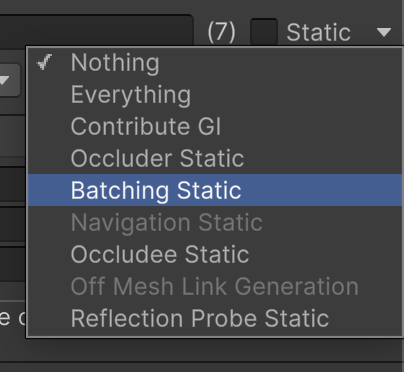
\includegraphics[width=0.5\textwidth]{immagini/cap2/unity_static_flag.png}
    \caption{Interfaccia di Unity nell'Inspector che mostra l'attivazione specifica del flag "Batching Static" per un oggetto statico.}
    \label{fig:unity_static_flag}
\end{figure}

Sebbene questo approccio aumenti l'utilizzo della memoria RAM, il vantaggio prestazionale è massimo: la CPU deve inviare un unico comando di disegno per l'intero gruppo, azzerando l'overhead di comunicazione per i singoli componenti.

\begin{lstlisting}[caption={Preprocessing logic for Static Batching.}]
// Initialization Phase (Build or Scene Load)
for each Material M in Scene:
    MeshList = FindStaticObjectsWith(M)
    CombinedMesh = new Mesh()
        
    for each Object in MeshList:
        // Transform vertices to world coordinates and merge
        WorldVertices = Object.mesh.TransformToWorldSpace()
        CombinedMesh.AddVertices(WorldVertices)
        
    // During Rendering Loop
    GPU.Draw(CombinedMesh, M)
\end{lstlisting}

\subsection{GPU Instancing} 

È la tecnica principale per renderizzare molteplici copie dello stesso modello geometrico utilizzando un set di dati condiviso \cite{AkenineRealTimeRendering}. A differenza del \textit{static batching}, questa tecnica non genera una nuova \textit{mesh} combinata; il motore invia alla GPU un'unica copia dei dati geometrici (vertici e indici) insieme a un \textit{array} di dati variabili, definiti \textit{per-instance data} (come matrici di trasformazione o variazioni di colore) \cite{UnityGPUInstancing}.

La GPU è quindi in grado di eseguire un ciclo di rendering interno estremamente efficiente, disegnando l'oggetto $N$ volte con una singola \textit{draw call}.

L'opzione deve essere esplicitamente abilitata nelle impostazioni del materiale.

\begin{figure}[H]
    \centering
    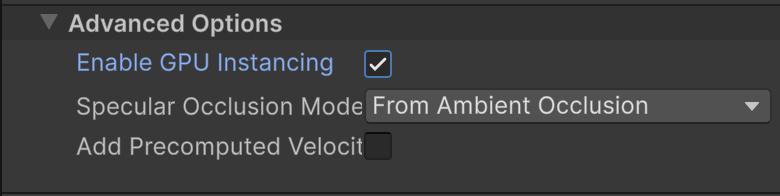
\includegraphics[width=0.7\textwidth]{immagini/cap2/gpu_instancing_flag.png}
    \caption{Abilitazione della spunta "Enable GPU Instancing" nelle "Advanced Options" di un materiale HDRP.}
    \label{fig:gpu_instancing_flag}
\end{figure}

    La logica di esecuzione a basso livello può essere schematizzata come segue:

\begin{lstlisting}[language=pseudo, caption={Algorithm for GPU Instancing execution.}, label={alg:gpu_instancing}]
// Prepare per-instance data arrays on CPU
TransformArray = [Pos1, Pos2, ... PosN]
PropertyArray  = [Color1, Color2, ... ColorN]

// Set the GPU state for the shared geometry
GPU.BindMesh(OriginalMesh)
GPU.BindMaterial(InstancedMaterial)

// Upload instance arrays to the GPU Constant Buffer
GPU.UploadToCBuffer(TransformArray, PropertyArray)

// Hardware-accelerated draw call for N instances
GPU.DrawInstanced(OriginalMesh, N)
\end{lstlisting}
    
\subsection{SRP Batcher} 
Rappresenta la tecnologia di punta per l'ottimizzazione in ambiente HDRP. A differenza delle tecniche di \textit{batching} tradizionali, che mirano esclusivamente a ridurre il numero assoluto di \textit{draw call}, l'SRP Batcher si focalizza sulla riduzione dei cambiamenti di stato tra una chiamata e l'altra. Questo avviene attraverso il raggruppamento di sequenze di comandi GPU di tipo \textit{bind} e \textit{draw} in quelli che vengono definiti \textit{SRP batch} \cite{UnitySRPBatcher}.
    
Il funzionamento del sistema si basa sulla persistenza dei dati dei materiali all'interno della memoria della GPU. L'SRP Batcher evita il caricamento ridondante dei dati se lo \textit{shader variant} rimane lo stesso.
    
\begin{figure}[H]
    \centering
    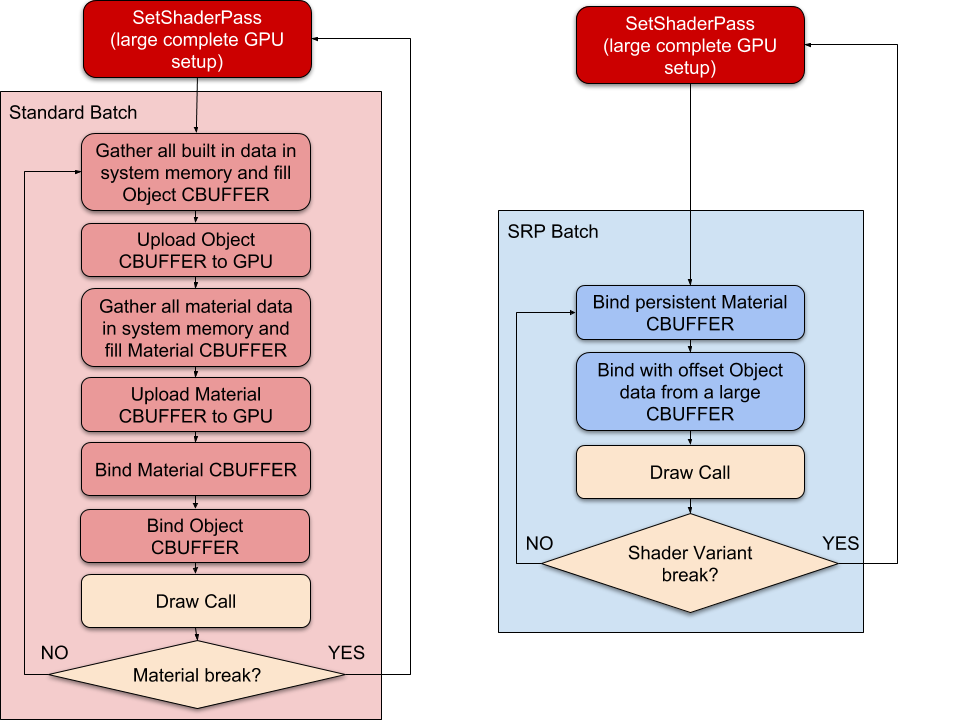
\includegraphics[width=0.85\textwidth]{immagini/cap2/SROShaderPass.png}
    \caption{Confronto tra il flusso di un batch standard e un SRP Batch.}
    \label{fig:srp_comparison}
\end{figure}
    
Dal punto di vista architettonico (Figura \ref{fig:srp_architecture}), quando il motore rileva un nuovo materiale, la CPU raccoglie tutte le proprietà e le lega alla GPU in appositi \textit{constant buffers} (CBUFFER). Se il contenuto del materiale non cambia, i dati persistono nella memoria video, rendendoli immediatamente pronti all'uso senza ulteriori interventi della CPU.
    
\begin{figure}[H]
    \centering
    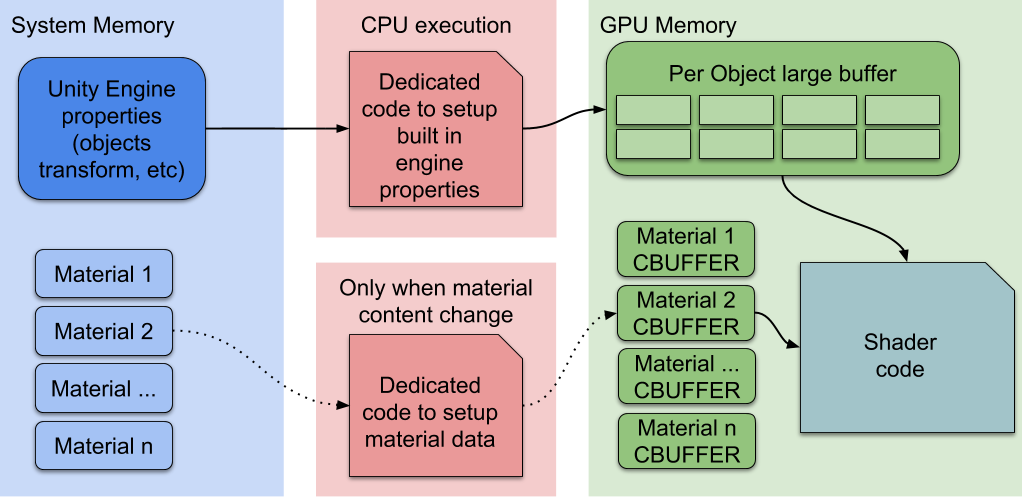
\includegraphics[width=0.9\textwidth]{immagini/cap2/SRP_Batcher_loop.png}
    \caption{Architettura della memoria nell'SRP Batcher.}
    \label{fig:srp_architecture}
\end{figure}
    
In questo scenario, il carico di lavoro del processore si riduce drasticamente, limitandosi alla gestione delle \textit{Unity Engine properties} (come le trasformazioni degli oggetti) all'interno di un unico grande buffer GPU (\textit{Per Object large buffer}).

\section{Shader: fondamenti teorici e linguaggio HLSL}

\subsection{Definizione di Shader}

Uno \textit{shader} è un programma, scritto in un linguaggio di alto livello, progettato per essere eseguito direttamente sulle unità di calcolo parallelo della GPU \cite{AkenineRealTimeRendering}. A differenza degli algoritmi eseguiti sulla CPU, che operano su flussi di dati generici, lo \textit{shader} ha il compito esclusivo di istruire il processore grafico su come trasformare i dati geometrici in informazioni visive (\textit{pixel}) \cite{HughesComputerGraphics}.

Il vantaggio fondamentale dello \textit{shader} risiede nell'architettura parallela della GPU: lo stesso codice viene eseguito contemporaneamente per migliaia di elementi diversi, garantendo una velocità di elaborazione che sarebbe impossibile da raggiungere con un'esecuzione sequenziale tradizionale.

\subsection{Classificazione degli Shader nella Pipeline Programmabile}

All'interno della moderna \textit{Graphics Pipeline}, le diverse fasi di elaborazione possono essere classificate in base alla loro flessibilità e necessità di implementazione da parte dello sviluppatore \cite{AkenineRealTimeRendering, ShirleyFundamentals}. Ogni blocco svolge una specifica funzione nel trasformare i dati in ingresso nell'immagine finale a schermo.

\begin{figure}[H]
    \centering
    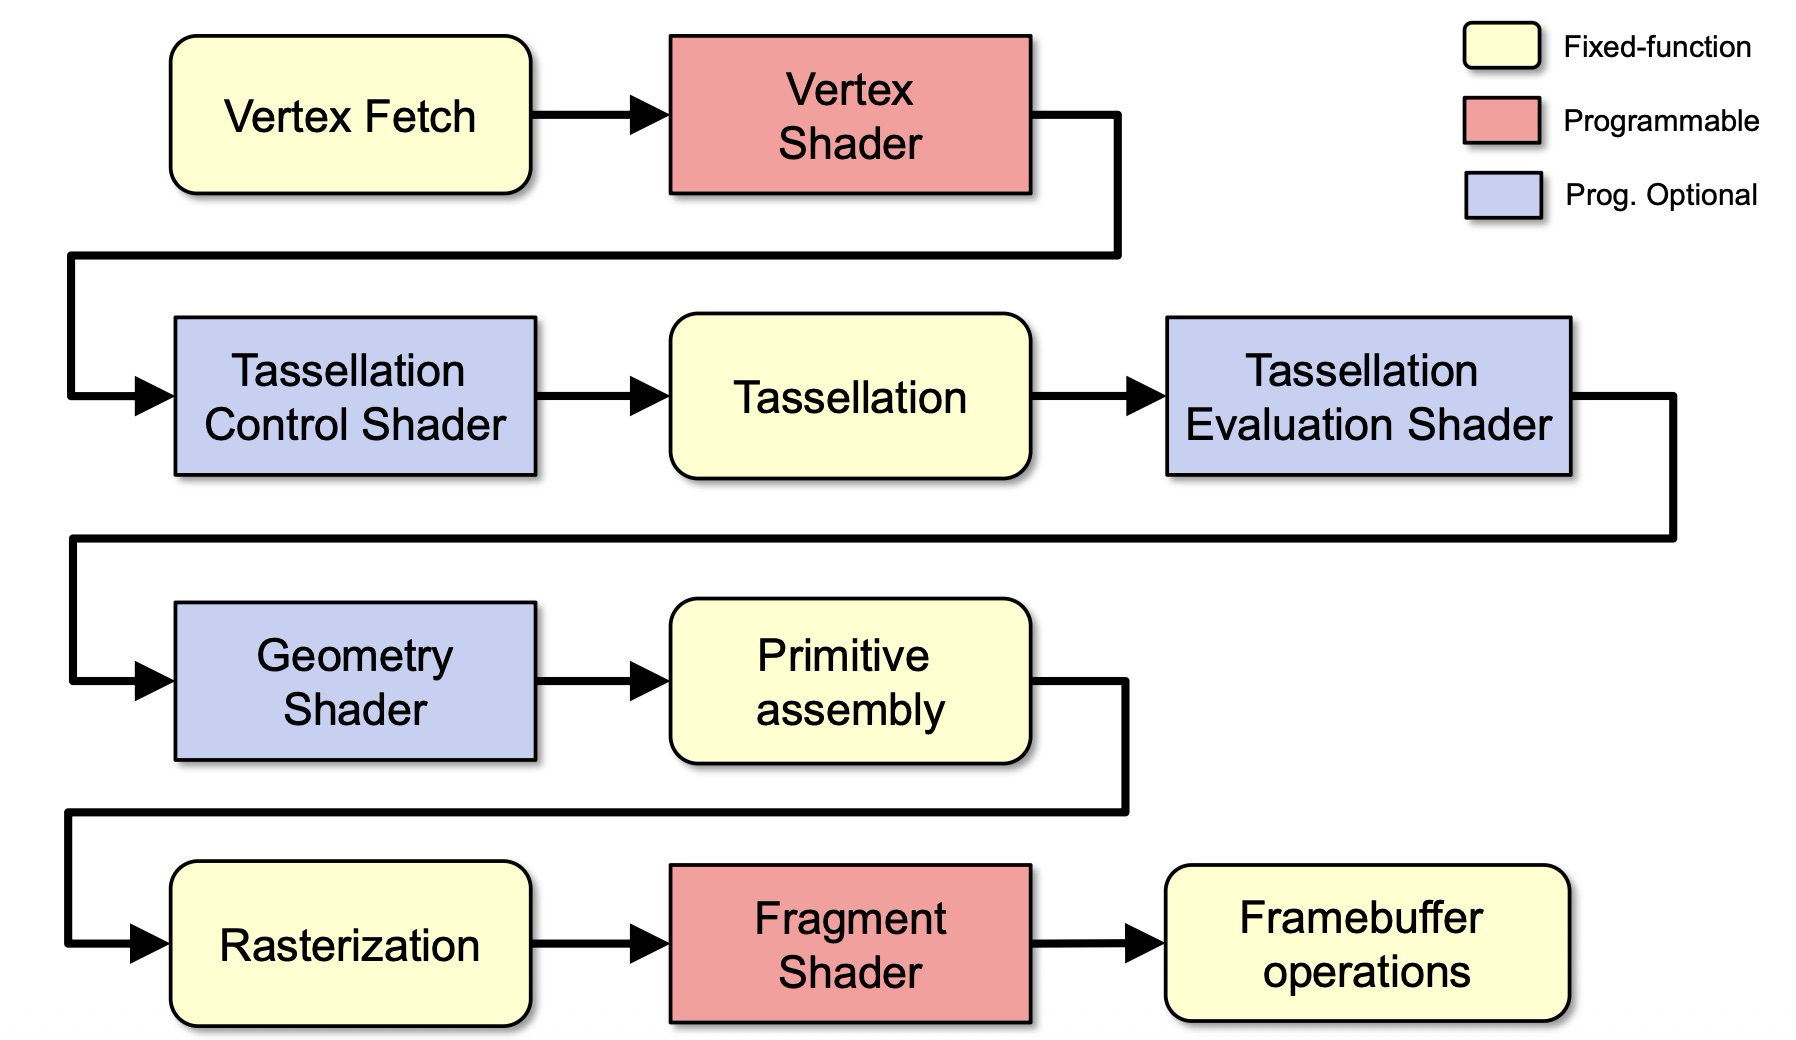
\includegraphics[width=\textwidth]{immagini/cap2/shaders_pipeline.png}
    \caption{Schema della Graphics Pipeline con distinzione tra blocchi fissi, programmabili e opzionali.}
    \label{fig:shaders_pipeline}
\end{figure}

Le macro-categorie che compongono l'architettura della pipeline sono:

\begin{itemize}
    \item \textbf{Blocchi Fissi:} Si tratta di fasi predefinite che utilizzano tecniche standard altamente ottimizzate a livello hardware. Non sono programmabili dall'utente e includono operazioni fondamentali come il \textit{Vertex Fetch}, la \textit{Tassellation} hardware e la \textit{Rasterization}.
    
    \item \textbf{Blocchi Programmabili:} Sono stadi che devono essere necessariamente implementati dallo sviluppatore attraverso la scrittura di appositi programmi chiamati \textit{Shader}. I due pilastri di questa categoria sono:
    \begin{itemize}
        \item \textbf{Vertex Shader:} Elabora ogni singolo vertice generandone gli attributi e applicando le trasformazioni geometriche necessarie per convertire le coordinate 3D nel sistema proiettivo.
        \item \textbf{Fragment Shader:} Riceve in input i frammenti generati dalla rasterizzazione e determina il colore effettivo di ogni pixel.
    \end{itemize}
    
    \item \textbf{Blocchi Programmabili Opzionali:} Rappresentano stadi aggiuntivi che vengono implementati solo se richiesto dalle specifiche necessità del rendering. Tra questi si distinguono:
    \begin{itemize}
        \item \textbf{Tassellation Control Shader (TCS):} Specifica il numero di vertici da generare per la suddivisone della primitiva.
        \item \textbf{Tassellation Evaluation Shader (TES):} Processa i nuovi vertici generati durante la fase di tassellazione.
        \item \textbf{Geometry Shader:} È in grado di modificare, eliminare o generare nuove primitive, cambiando potenzialmente la topologia della mesh (ad esempio, trasformando triangoli in linee).
    \end{itemize}
\end{itemize}

L'interazione tra questi blocchi permette un controllo granulare su ogni fase del rendering, partendo dal \textit{Vertex Fetch} dei dati (posizione 3D, vettori normali, colori e coordinate di \textit{texture}) fino alle operazioni finali sul \textit{Framebuffer}, dove i frammenti subiscono test di visibilità e profondità prima di essere scritti a schermo \cite{AkenineRealTimeRendering, HughesComputerGraphics}.
